\documentclass[ignorenonframetext,aspectratio=169]{beamer}
\setbeamertemplate{caption}[numbered]
\setbeamertemplate{caption label separator}{: }
\setbeamercolor{caption name}{fg=normal text.fg}
\beamertemplatenavigationsymbolsempty
\usepackage{lmodern}
\usepackage{amssymb,amsmath}
\usepackage{ifxetex,ifluatex}
\usepackage{fixltx2e} % provides \textsubscript
\ifnum 0\ifxetex 1\fi\ifluatex 1\fi=0 % if pdftex
  \usepackage[T1]{fontenc}
  \usepackage[utf8]{inputenc}
\else % if luatex or xelatex
  \ifxetex
    \usepackage{mathspec}
  \else
    \usepackage{fontspec}
  \fi
  \defaultfontfeatures{Ligatures=TeX,Scale=MatchLowercase}
\fi
% use upquote if available, for straight quotes in verbatim environments
\IfFileExists{upquote.sty}{\usepackage{upquote}}{}
% use microtype if available
\IfFileExists{microtype.sty}{%
\usepackage{microtype}
\UseMicrotypeSet[protrusion]{basicmath} % disable protrusion for tt fonts
}{}
\newif\ifbibliography
\usepackage{graphicx,grffile}
\makeatletter
\def\maxwidth{\ifdim\Gin@nat@width>\linewidth\linewidth\else\Gin@nat@width\fi}
\def\maxheight{\ifdim\Gin@nat@height>\textheight0.8\textheight\else\Gin@nat@height\fi}
\makeatother
% Scale images if necessary, so that they will not overflow the page
% margins by default, and it is still possible to overwrite the defaults
% using explicit options in \includegraphics[width, height, ...]{}
\setkeys{Gin}{width=\maxwidth,height=\maxheight,keepaspectratio}

% Prevent slide breaks in the middle of a paragraph:
\widowpenalties 1 10000
\raggedbottom

\AtBeginPart{
  \let\insertpartnumber\relax
  \let\partname\relax
  \frame{\partpage}
}
\AtBeginSection{
  \ifbibliography
  \else
    \let\insertsectionnumber\relax
    \let\sectionname\relax
    \frame{\sectionpage}
  \fi
}
\AtBeginSubsection{
  \let\insertsubsectionnumber\relax
  \let\subsectionname\relax
  \frame{\subsectionpage}
}

\setlength{\emergencystretch}{3em}  % prevent overfull lines
\providecommand{\tightlist}{%
  \setlength{\itemsep}{0pt}\setlength{\parskip}{0pt}}
\setcounter{secnumdepth}{0}
\DeclareUnicodeCharacter{1D53D}{\mathbb{F}}
\DeclareUnicodeCharacter{2234}{$\therefore$}
\DeclareUnicodeCharacter{2228}{$\vee$}
\DeclareUnicodeCharacter{2227}{$\wedge$}
\DeclareUnicodeCharacter{2124}{\mathbb{Z}}
\DeclareUnicodeCharacter{03C9}{$\omega$}
\DeclareUnicodeCharacter{03B5}{$\varepsilon$}
\DeclareUnicodeCharacter{03B4}{$\delta$}
\DeclareUnicodeCharacter{00A0}{~}
\hypersetup{colorlinks,linkcolor=,urlcolor=purple}
\setbeamertemplate{navigation symbols}{}
\setbeamercolor{footnote mark}{fg=gray}
\setbeamerfont{footnote}{size=\tiny}
\usefonttheme[onlymath]{serif}

\title{Controlling the mine fire}
\subtitle{The CA industry in 2016 and beyond}
\author{Fraser Tweedale\\
    \texttt{@hackuador}}
\date{February 25 2017}

\begin{document}
\frame{\titlepage}

\begin{frame}{~~}

\begin{center}
\def\svgwidth{.5\paperheight}
\input{identity-secure-ARTIFACT.pdf_tex}
\end{center}

\end{frame}

\begin{frame}{This talk}

\begin{itemize}
\tightlist
\item
  Overview of CA industry
\item
  Explain some mishaps of last couple years
\item
  Overview of some efforts to make things less bad
\item
  Recommendations; what \emph{you} can do right now
\end{itemize}

\end{frame}

\begin{frame}{Certificate Authorities and TLS}

\begin{itemize}
\tightlist
\item
  CAs issue certificates that \textbf{bind public keys to domains}

  \begin{itemize}
  \tightlist
  \item
    Usually for \$\$\$
  \end{itemize}
\item
  A \textbf{server} presents its certificate during TLS handshake
\item
  Client (browser) validates certificate against \textbf{trusted CAs}
\end{itemize}

\end{frame}

\begin{frame}{~~}

\begin{center}
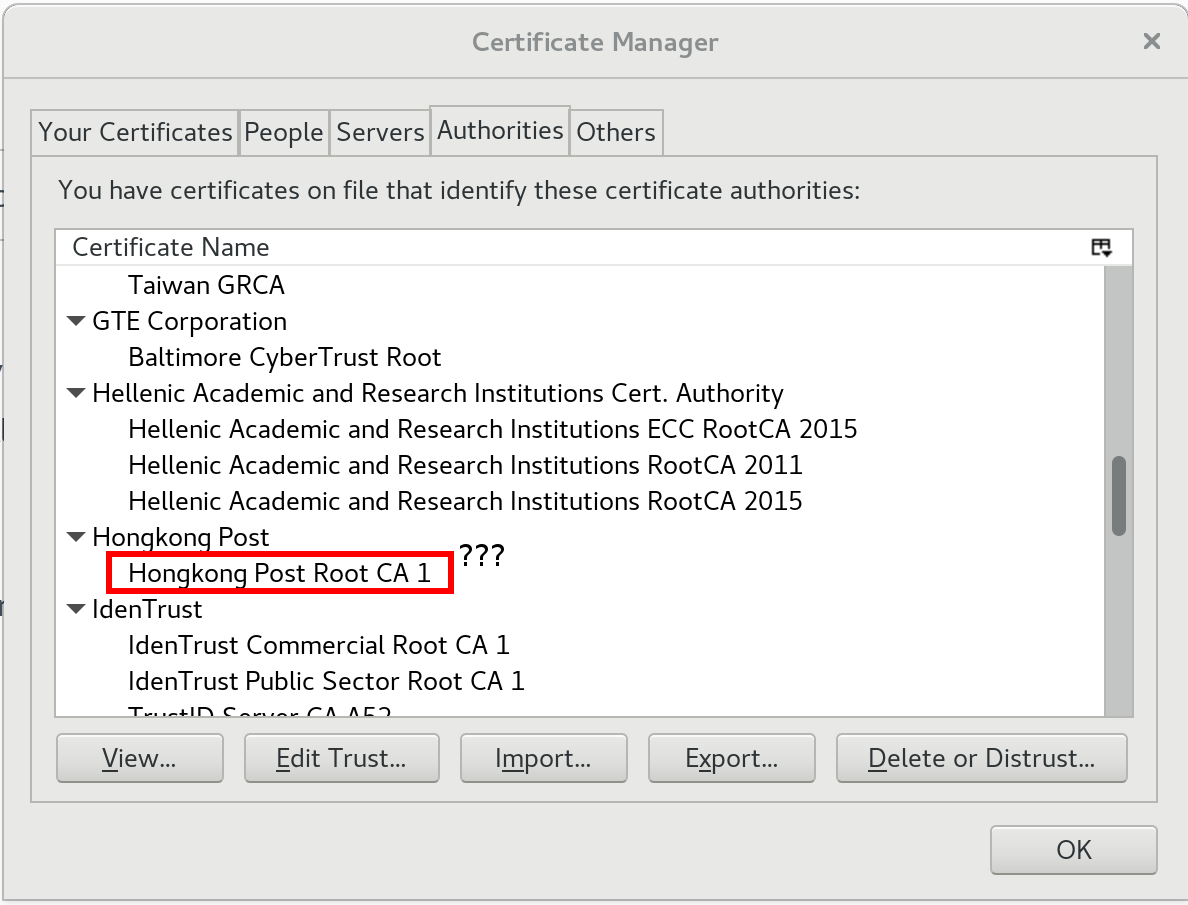
\includegraphics{ff-cas.png}
\end{center}

\end{frame}

\begin{frame}{What's wrong with the CA industry?}

\begin{itemize}
\tightlist
\item
  Literally hundreds of trusted CAs
\item
  We can't possibly audit them all properly
\item
  Business model does not encourage disclosure of problems
\item
  Basically it's a shakedown
\end{itemize}

\end{frame}

\begin{frame}{~~}

\begin{center}
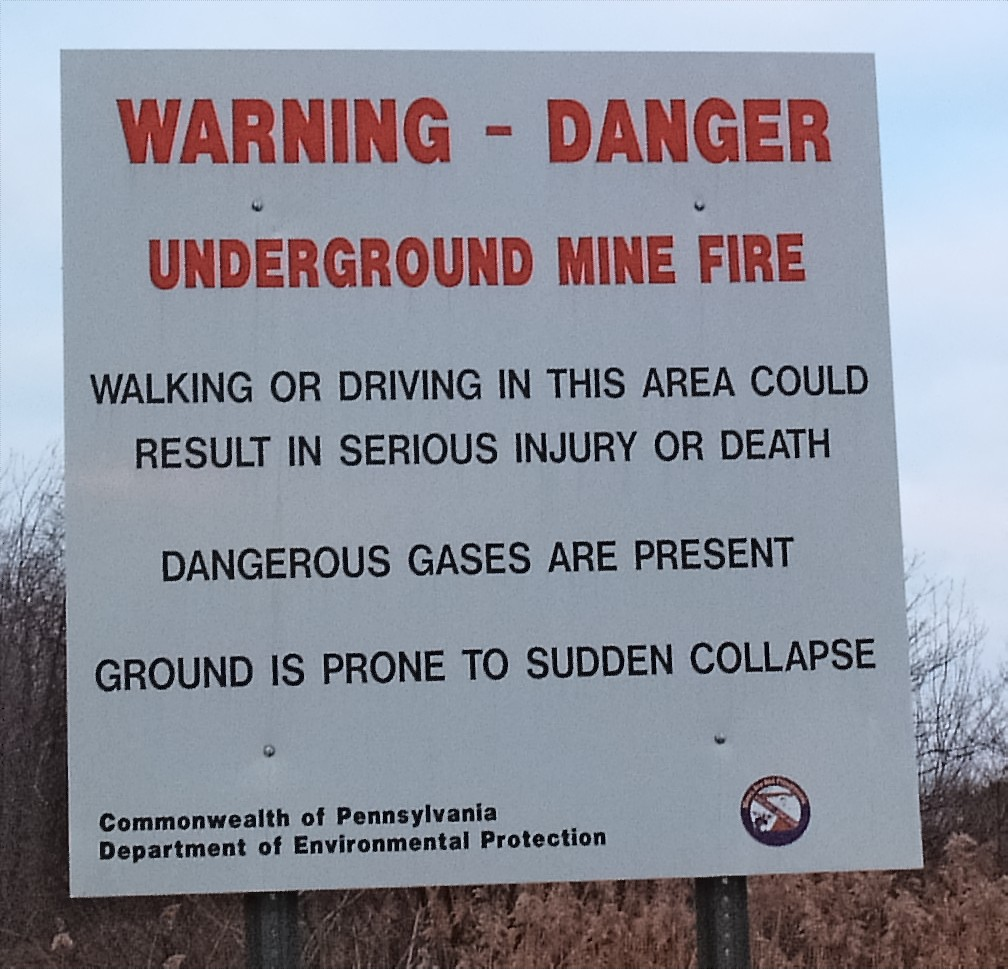
\includegraphics{Censign.jpg}
\end{center}

\end{frame}

\begin{frame}{2016: WoSign / StartCom}

\begin{itemize}
\item Background: SHA-1 certs prohibited from 1 Jan 2016\footnote[frame]{
  \url{https://cabforum.org/2014/10/16/ballot-118-sha-1-sunset/}}
\item WoSign got caught "backdating" certs to get around this\footnote[frame]{
  \url{https://wiki.mozilla.org/CA:WoSign_Issues}}
\item Several other issues
  \begin{itemize}
  \item failed to disclose purchase of StartCom
  \item unverified info in subject name
  \end{itemize}
\end{itemize}

\end{frame}

\begin{frame}{2015: Symantec}

\begin{itemize}

\item Sept 14: Symantec {\em Thawte} CA issued certs for
  {\tt google.com}\footnote{\url{https://security.googleblog.com/2015/09/improved-digital-certificate-security.html}}

\item Further investigation turned up 1000s of misissued
  certs\footnote{\url{https://security.googleblog.com/2015/10/sustaining-digital-certificate-security.html}}

\end{itemize}

\end{frame}

\begin{frame}{2017: Symantec}

\begin{itemize}

\item January 19: 108 more misissued certs
  discovered\footnote{\url{https://www.mail-archive.com/dev-security-policy@lists.mozilla.org/msg05455.html}}

\item After 2015 incidents, Symantic claimed to have implemented
  controls to prevent future
  misissuance...\footnote{\url{https://www.symantec.com/page.jsp?id=test-certs-update}}

\end{itemize}

\end{frame}

\begin{frame}{~~}

\begin{center}
\def\svgwidth{.7\textwidth}
\input{letsencrypt-logo-horizontal-ARTIFACT.pdf_tex}
\end{center}

\end{frame}

\begin{frame}{Let's Encrypt - overview}

\begin{itemize}
\tightlist
\item
  free, automated, publicly trusted CA
\item
  domain validation only (this is fine)
\item
  ACME protocol
\item
  went live in \textbf{November 2015}
\end{itemize}

\end{frame}

\begin{frame}{Let's Encrypt - impact}

\begin{center}
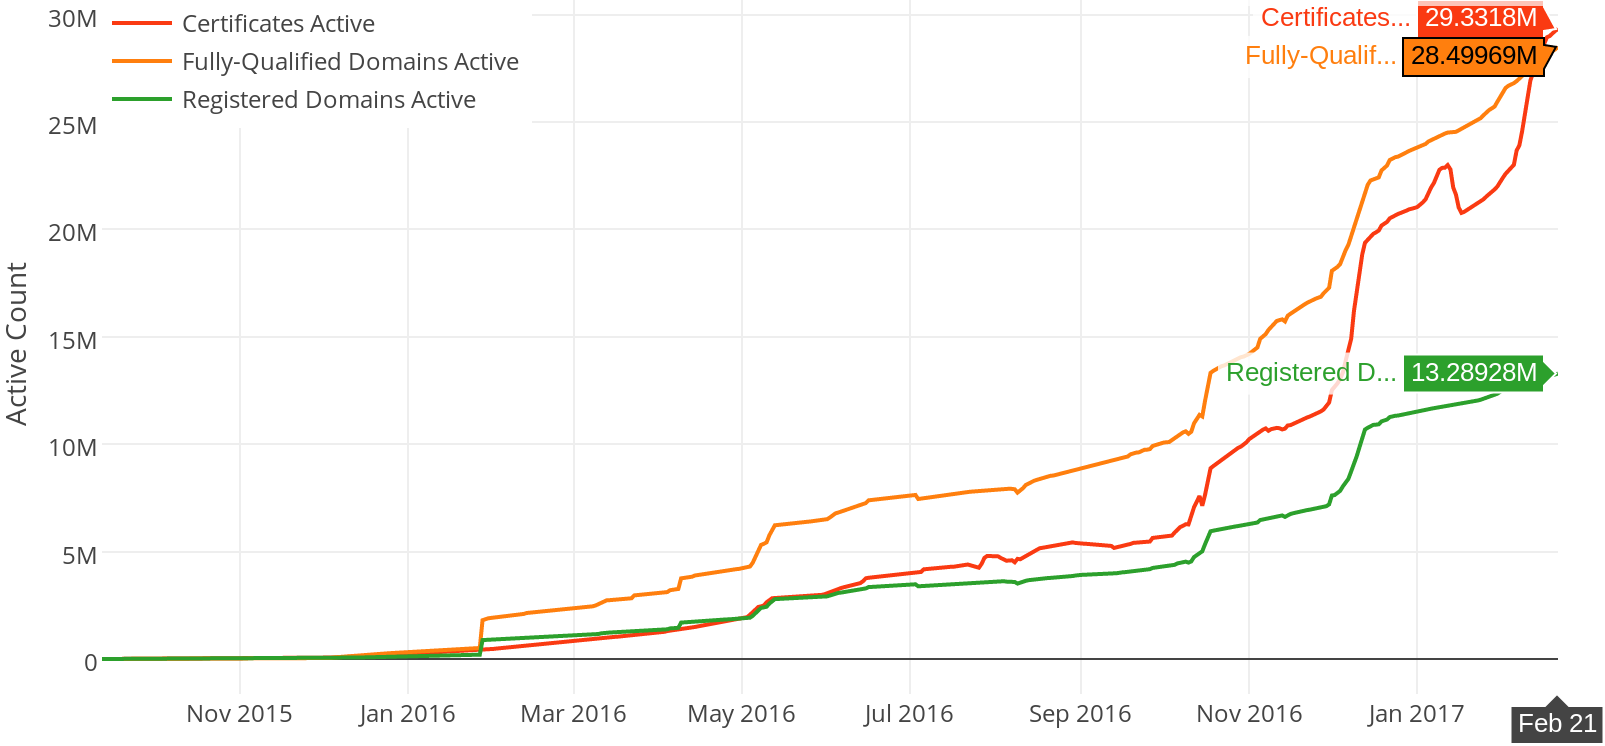
\includegraphics{le-growth.png}
\end{center}

\tiny

\url{https://letsencrypt.org/stats/}

\end{frame}

\begin{frame}{Let's Encrypt - impact}

\begin{itemize}

\item 3rd biggest CA by certs issued

\item 93\% of domains never previously had a
  cert\footnote{\url{https://arxiv.org/pdf/1612.03005.pdf}}

\item 47\% LE certs issued to 3 hosting providers
  \begin{itemize}
  \item WordPress, Shopify, OVH
  \end{itemize}

\item Firefox \% page loads HTTPS
  \begin{itemize}
  \item November 2015: 40\%
  \item November 2016: {\bf 50\%}
  \end{itemize}

\end{itemize}

\end{frame}

\begin{frame}{~~}

\begin{center}
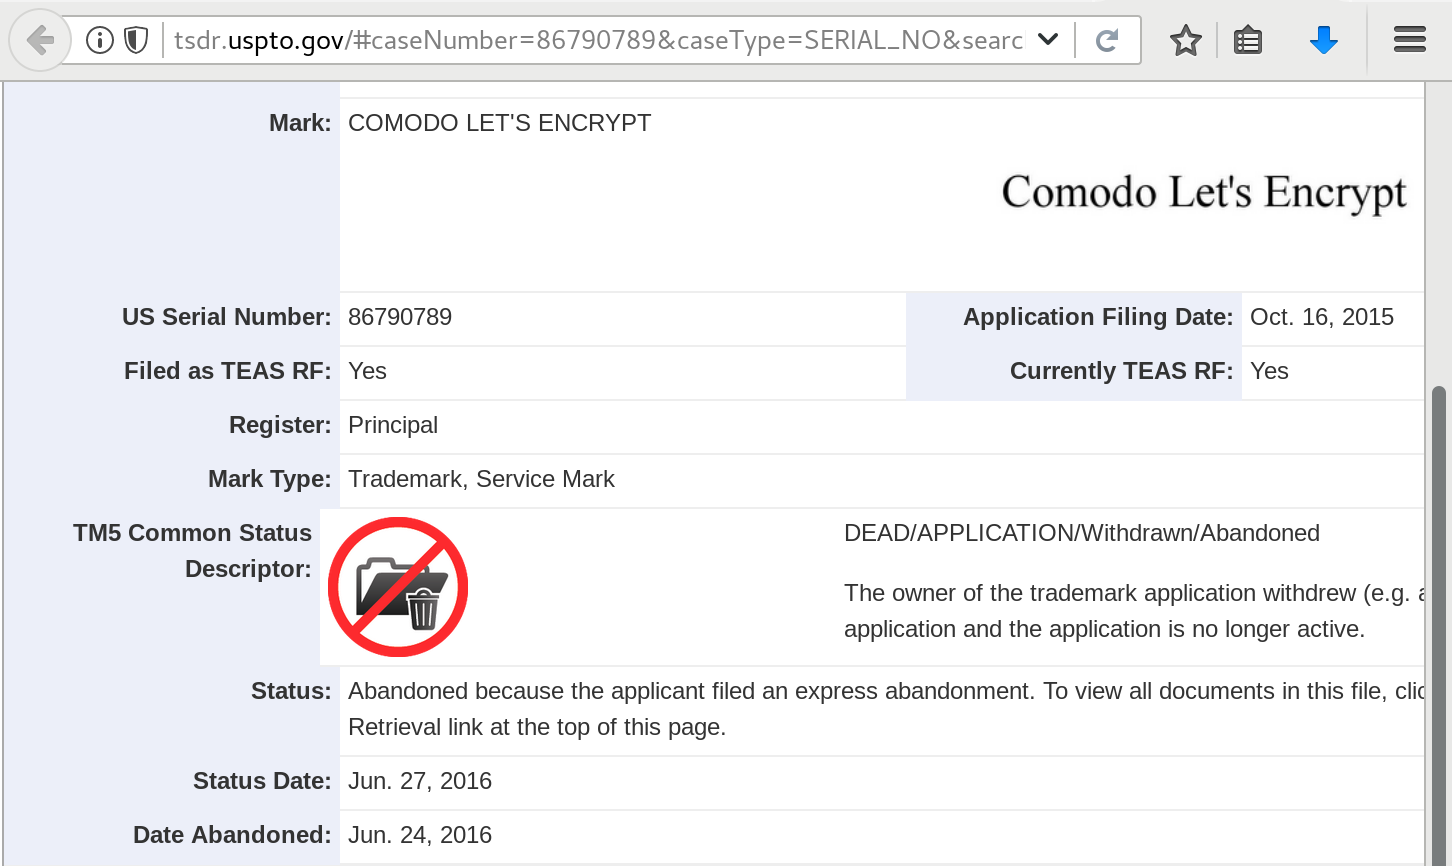
\includegraphics{comodo-lets-encrypt.png}
\end{center}

\end{frame}

\begin{frame}{Comodo vs Let's Encrypt}

\begin{itemize}

\item Comodo filed 3 trademark applications, Oct 2015

  \begin{itemize}
  \item  ISRG had been using *Let's Encrypt* since Nov 2014
  \end{itemize}

\item  Engaged Comodo privately from March 2016

\item  ISRG went public
  June 23...\footnote{\url{https://letsencrypt.org/2016/06/23/defending-our-brand.html}}

\item<+->  June 24: Comodo abandons applications

\end{itemize}

\end{frame}

\begin{frame}{Comodo vs Let's Encrypt}
\large
\begin{quote}
  Trying to piggy back on our business model and copying our model
  of giving certificates for 90 days for free is not ethical. They
  clearly wanted to leverage the market of Free SSL users we had
  helped create and establish and that's why they created exactly
  same 90 day free ssl offering.\\
  ~~~~~~~~~~~~~~~~~~~~~~~~---Melih Abdulhayoglu, Comodo CEO
\end{quote}

\bigskip

\tiny

\url{https://forums.comodo.com/general-discussion-off-topic-anything-and-everything/shame-on-you-comodo-t115958.0.html}

\end{frame}

\begin{frame}{StartCom/WoSign vs Let's Encrypt}

\begin{itemize}
\tightlist
\item
  \textbf{\emph{StartEncrypt}} announced 6 June 2016
\item
  full of security holes

  \begin{itemize}
  \tightlist
  \item
    attacker-controlled path for DV check
  \item
    duplicate signature key selection attack
  \item
    private key mode 0666
  \end{itemize}
\item
  abandoned 4 July; moving to ACME
\end{itemize}

\end{frame}

\begin{frame}{~~}

\begin{center}
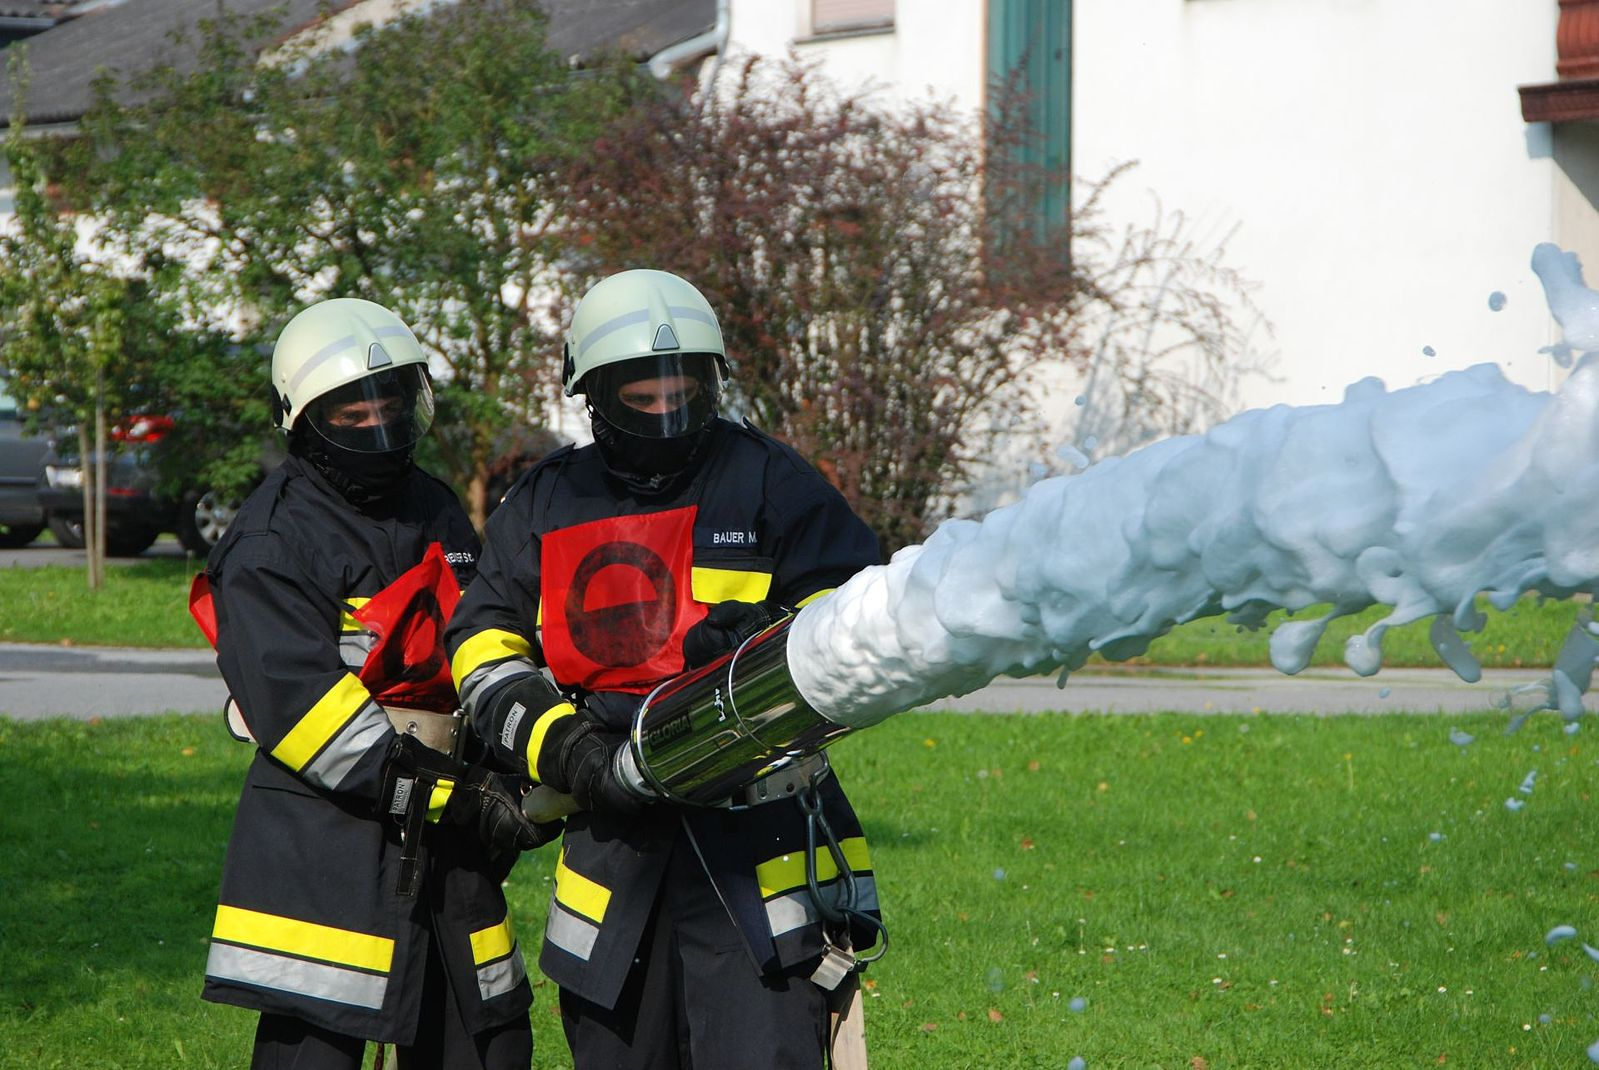
\includegraphics{FF_Loeschuebung_mit_Mittelschaum.jpg}
\end{center}

\tiny

CC BY-SA 3.0
\url{https://commons.wikimedia.org/wiki/File:FF_Loeschuebung_mit_Mittelschaum.jpg}

\end{frame}

\begin{frame}{Certificate Transparency}

\begin{itemize}
\tightlist
\item
  Append-only, immutable log of observed certificates
\item
  Can be monitored by CAs themselves, domain owners, etc.
\item
  Enables early detection of misissued certs, infra hijack
\end{itemize}

\end{frame}

\begin{frame}{~~}

\begin{center}
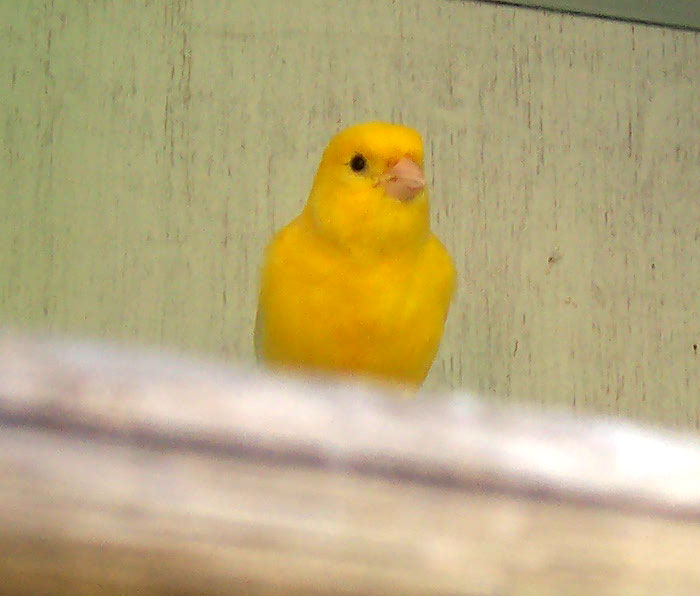
\includegraphics{Canary.jpg}
\end{center}

\tiny

CC BY-SA 3.0 \url{https://commons.wikimedia.org/wiki/File:Canary.jpg}

\end{frame}

\begin{frame}{~~}

\begin{center}
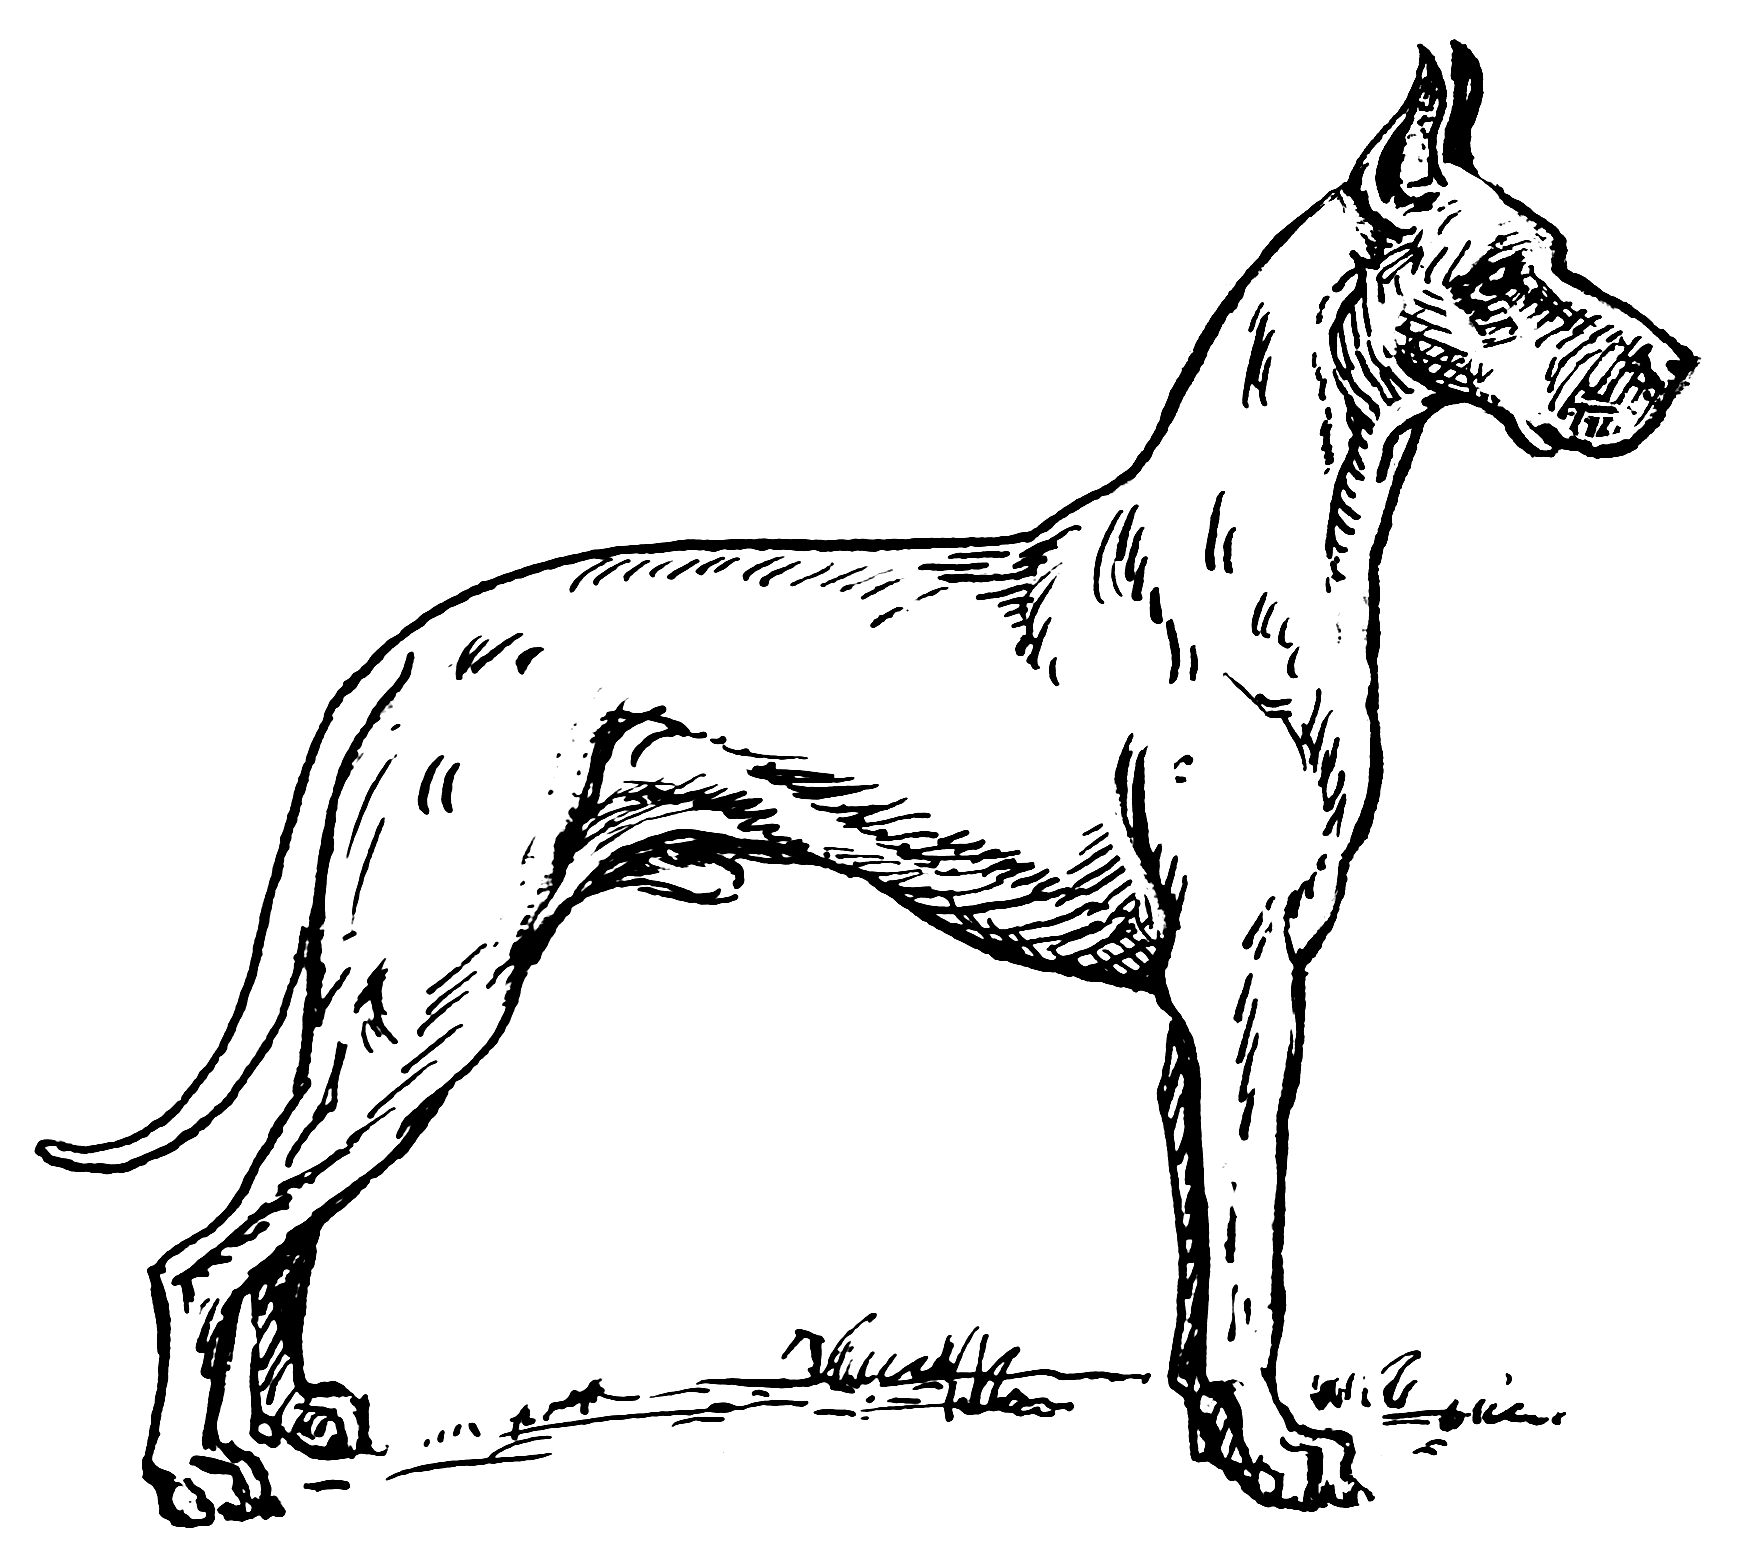
\includegraphics{Great_Dane_(PSF).png}
\end{center}

\tiny

CC BY-SA 3.0 \url{https://commons.wikimedia.org/wiki/File:Canary.jpg}

\end{frame}

\begin{frame}{DANE}

\begin{itemize}
\tightlist
\item
  \emph{DNS-Based Authentication of Named Entities} (RFC 6698)
\item
  end-run around the CA industry
\item
  certs, CA certs or fingerprints in DNS(SEC)
\item
  key endorsement rests with domain owner
\item
  tradeoff: absolute trust in a DNSSEC root key
\end{itemize}

\end{frame}

\begin{frame}{Browser/OS vendors flex their muscle}

\begin{itemize}
\item WoSign/StartCom distrusted\footnote[frame]{
  \url{https://blog.mozilla.org/security/2016/10/24/distrusting-new-wosign-and-startcom-certificates/}}
\item Chrome to require CT for certs issued after Oct 2017\footnote[frame]{
  \url{https://groups.google.com/a/chromium.org/forum/\#!msg/ct-policy/78N3SMcqUGw/ykIwHXuqAQAJ}}
\item Pushing to limit cert lifetimes to 13 months\footnote{
  \url{https://cabforum.org/pipermail/public/2017-February/009530.html}}
\end{itemize}

\end{frame}

\begin{frame}{What can \emph{you} do about it?}

\begin{itemize}
\tightlist
\item
  use, implement, support Let's Encrypt
\item
  use Strict Transport Security (HSTS); consider preload
\item
  use key pinning (HPKP, minimal trust stores, etc)
\item
  monitor CT logs for your domains
\item
  deploy DNSSEC; prepare for DANE
\end{itemize}

\end{frame}

\begin{frame}{Fin}

\begin{columns}

  %\begin{column}{.4\textwidth}
  %  put something here? % \includegraphics[width=1.2\textwidth]{FILENAME}
  %\end{column}

  %\begin{column}{.6\textwidth}

    \setlength{\parskip}{.5em}

    { \centering

    \input{cc-by-ARTIFACT.pdf_tex}

    \copyright~2017  Fraser Tweedale

    { \scriptsize
    Except where otherwise noted this work is licensed under
    }
    { \footnotesize
    \textbf{http://creativecommons.org/licenses/by/4.0/}
    }

    }

    \begin{description}
    \item[Twitter]
    \texttt{@hackuador}
    \item[Email]
    \texttt{frase@frase.id.au}
    \end{description}
  %\end{column}

\end{columns}

\end{frame}

\end{document}
